% Sample apostrophy's to remove team's 

\title{Lessons Learned from an Extended Participant Observation Grounded Theory Study}

\author{
\IEEEauthorblockN{ Todd Sedano }
\IEEEauthorblockA{Pivotal Software \\
  Palo Alto, CA \\
  Carnegie Mellon University \\
  Silicon Valley Campus \\  
  Email: professor@gmail.com}
\and
\IEEEauthorblockN{ Paul Ralph }
\IEEEauthorblockA{University of Auckland \\
  Auckland, New Zealand}
\IEEEauthorblockA{University of British Columbia \\
  Vancouver, BC, Canada \\
  Email: paul@paulralph.name}
\and
\IEEEauthorblockN{ C\'ecile P\'eraire }
\IEEEauthorblockA{Carnegie Mellon University \\
  Electrical and Computer Engineering \\
  Silicon Valley Campus \\
  Moffett Field, CA 94035, USA \\
  Email: cecile.peraire@sv.cmu.edu}
}
% make the title area
\maketitle

\section*{Abstract}
\textit{Context:} Conducting a Grounded Theory study is rigorous, demanding, and challenging. Misperceptions exist within the software engineering community \cite{StolGroundedTheory}.

\textit{Objective:} The purpose of this paper is to describe one extended participant observation Grounded Theory study for aiding new empirical researchers wanting to run similar research studies.

\textit{Method:} Following Constructivist Grounded Theory, we conducted a \durationOfResearchStudy{} participant-observation of \numberOfObservedProjects{} software development projects at Pivotal, a software development organization, interviewed \numberOfInterviews{} software engineers, interaction designers, and product managers, and analyzed one year of retrospection topics. We iterated between analysis and theoretical sampling until achieving theoretical saturation, publishing papers on team code ownership \cite{SedanoTeamCodeOwnership}, sustainable software development through overlapping code ownership \cite{SedanoSustainableSoftware}, and software development waste \cite{SedanoSoftwareDevelopmentWaste}. 

\textit{Results:} This paper describes the mis-steps, challenges, and unique insights that occurred while conducting a Grounded Theory study.

\textit{Limitations:} While the process and results are highly relevant to the researcher, the outcomes might not apply to other researchers.

\textit{Conclusion:} Conducting my own Grounded Theory research study, attending Glaser's Seminar, and reading and re-reading Charmaz's and Glaser's books helped the researcher overcoming misperceptions about Grounded Theory research.
\section{Introduction}
For the past 2.5 years, I \footnote{We have written this paper in the first person because it predominantly recounts the experience of the first author and because its narrative elements flow better this way.} have been conducting a full-time, participant observation, Grounded Theory study. Participant observation is a data collection method where the researcher participates in the project or organization being observed \cite{Trochim2006ResearchMethods}. Grounded Theory is a comprehensive research methodology that generates theory from observations \cite{GlaserDiscovery}. 

My first introduction to Grounded Theory came while reading Brown \cite{BreneBrownDaringGreatly} in March 2013. Brown details her journey in applying Grounded Theory to her psychological research about processing shame. Grounded Theory's focus on interpersonal communication appealed to me. Later, in May, I attended the first International Workshop on Conducting Empirical Studies in Industry (CESI 2013) and quizzed attendees about how they used Grounded Theory in their research. (Thanks to Irit Hadar and Christopher Bull for answering all of my questions.) During the main conference, (The 35th International Conference on Software Engineering), I attended each Grounded Theory presentation to learn more about how the community used the method.

Lengthy participant observation studies are unusual in software engineering and in computer science more generally. Moreover, software engineering contexts present unique, unresolved challenges for longitudinal participant observation and Grounded Theory \cite{StolGroundedTheory}. The purpose of this paper is therefore to offer guidance, based on my experiences, for researchers considering a similar trajectory. While we should avoid overgeneralizing from a sample of one, others may benefit from some ideas to try and possible risks to keep in mind. 

Grounded Theory is such a simple method, yet so easily and often misapplied \cite{StolGroundedTheory}. It is easy to describe but hard to understand. My Grounded Theory study appears typical: confusion followed by insight. A researcher starts a Grounded Theory study open to see where the research leads. Once unleashed, the method seems to have a mind of its own as it guides the researcher towards research treasure through uncharted territory. I've been teaching and performing Extreme Programming for over 11 years, yet the method delighted me by finding precious insights 

The structure of the paper follows the stages of a Grounded Theory study, Section \ref{GettingStarted} \quotes{Getting started,} Section \ref{ConstantComparison} \quotes{Constant Comparison,} Section \ref{TheoryConstruction} \quotes{Theory Construction,} Section \ref{TheoreticalSaturation} \quotes{Theoretical Saturation, }  Section \ref{ManagingTheData} \quotes{Managing The Data,}  Section \ref{Publishing} \quotes{Publishing,} Section \ref{AdvantagesDisadvantages} \quotes{Advantages and Disadvantages of Extended Participant Observation,} and  Section \ref{Conclusion} \quotes{Conclusion.}
\section{Getting Started}
\label{GettingStarted}

Following Glaser's advice of \quotes{just do it} \cite{GlaserIssues}, I learned the intricacies of Grounded Theory by diving into a study and reading about the methodology as I went. This section examines early important decisions such as which variant to use, selecting a site, and gathering rich data.
\subsection{Selecting a Method Variant}
Grounded Theory has many variants with both practical and philosophical differences. Initially, I chose Constructivist Grounded Theory simply because it was the latest, a fine justification for selecting software libraries, but as I later discovered, not the best reason for selecting a sociological research method. 

We continue to use Constructivist Grounded Theory for several reasons. Glaser's recommendations are not always practical (or acceptable in our community of practice); for instance, simply taking notes without recording/transcribing interviews and delaying the literature review until near the end of the study. Furthermore, a constructivist epistemology offers many advantages over Classic Grounded Theory's objectivist epistemology for software engineering contexts. Software development is a socio-technical endeavor. Many concepts software engineering researchers study are socially constructed (e.g. code, comments, tests, projects, schedules, teams). Moreover, software developers can be quite reflective and helpful in contributing to the construction of concepts. Constructivist Grounded Theory better acknowledges socially constructed concepts and participants' contribution to theorizing than many other Grounded Theory variants. 

\textit{Recommendation:} If you want to just get started, begin with Stol's comparison of the three variants \cite{StolGroundedTheory}, read a few exemplars (e.g. \cite{SedanoSustainableSoftware, SedanoSoftwareDevelopmentWaste}), and then read Charmaz's book \cite{Charmaz}. If you want more depth about each variant, read Evan's article \cite{Evans2013novice}. Note that Evan includes Glaser's pontificating criticisms of Constructivist Grounded Theory \cite{GlaserConstructivistGroundedTheory}, but excludes Bryant's rebuttal \cite{Bryant2007}. 

My primary text was Charmaz \cite{Charmaz}, which I supplemented with Glaser's books \cite{GlaserDiscovery, GlaserTheoreticalSensitivity, GlaserIssues} to build a deeper understanding of the method and the historical context of Constructivist Grounded Theory. I find Charmaz's writing more approachable and less polemical than Glaser's. 

\textit{Lesson Learned:} I initially read Glaser's books in the wrong sequence. His works are additive and build on each other.

\textit{Recommendation:} Read Glaser's books in order of publication, oldest first. 
\subsection{Selecting a Research Site}
Pivotal Labs is a division of Pivotal\textemdash a large American software company (with 17 offices around the world). Pivotal Labs provides teams of agile developers, product managers, and interaction designers to other firms. Its mission is not only to deliver highly-crafted software products but also to help transform clients' engineering cultures. To change the client's development process, Pivotal combines the client's software engineers with Pivotal's engineers at a Pivotal office where they can experience Extreme Programming \cite{BeckExtremeProgramming2004} in an environment conducive to agile development. Pivotal Labs has followed Extreme Programming \cite{BeckExtremeProgramming2004} since the late 1990's. 

We selected Pivotal because: 1) it is successful; 2) it is interesting in its continued use and evolution of extreme programming; 3) it is accessible and cooperative with research. Both Classic and Constructivist Grounded Theory advocate picking an interesting site to see \quotes{What's going on here?} 

\textit{Lessons learned:} Selecting a consultancy was helpful in several ways. Gaining insight into Pivotal Labs' way of working aligns with its business goals. They were therefore open to research provided we did not reveal information about clients. The client owns the code, not the way of working. Furthermore, a consultancy provides exposure to many different projects, both greenfield and brownfield. Client-Pivotal dynamics revealed tensions in adopting agile software development. However, the consultancy's focus on billing 40 hours per person per week limited research activities (e.g. data collection, data analysis, and attending conferences) to personal time.

\textit{Recommendation:} Since Grounded Theory starts with the question, \quotes{what is going on here?} start with an organization that excels at what you hope to research. Consultancies can work well. Try to negotiate a 20-30 hour per week contract so you have time reserved for research.
\subsection{Gathering Rich Data}
Initially, the two main data sources were interviews with Pivotal employees and notes on participant observation. We began with no solid expectations about the number of interviews or amount of participant observation that I would conduct. The interviewees consisted of interaction designers, product managers, and software engineers who had experience with Pivotal's software development process from five different Pivotal offices. At first, interviewees were selected opportunistically; for example, if a product manager visited from another office, I requested an interview. When I visited the Los Angeles area, I scheduled interviews at the Santa Monica office. 

\textit{Lesson learned:} Opportunistic interviewing sometimes generated an analysis backlog. 

\textit{Recommendation:} Prioritize analysis over data collection. 

I relied focused on \quotes{intensive interviews,} which are \quotes{open-ended yet directed, shaped yet emergent, and paced yet unrestricted} \cite{Charmaz}, to abandon assumptions and better understand the interviewee's perspective. This influenced the type of data I collected for participant observation. 

\textit{Lesson Learned:} Creating an interview guide helped me generate open-ended questions. Transcribing and coding my interviews enabled me to hear when I asked leading questions.

\textit{Recommendation:} Use an interview guide at most three times between revisions. This reinforces constant comparison and theoretical sampling. 

I asked early interviewees to draw their \quotes{view of Pivotal's software development process.} Figure \ref{2015_08_12_detailed} shows one response. 
\begin{figure}[htbp]
\centering
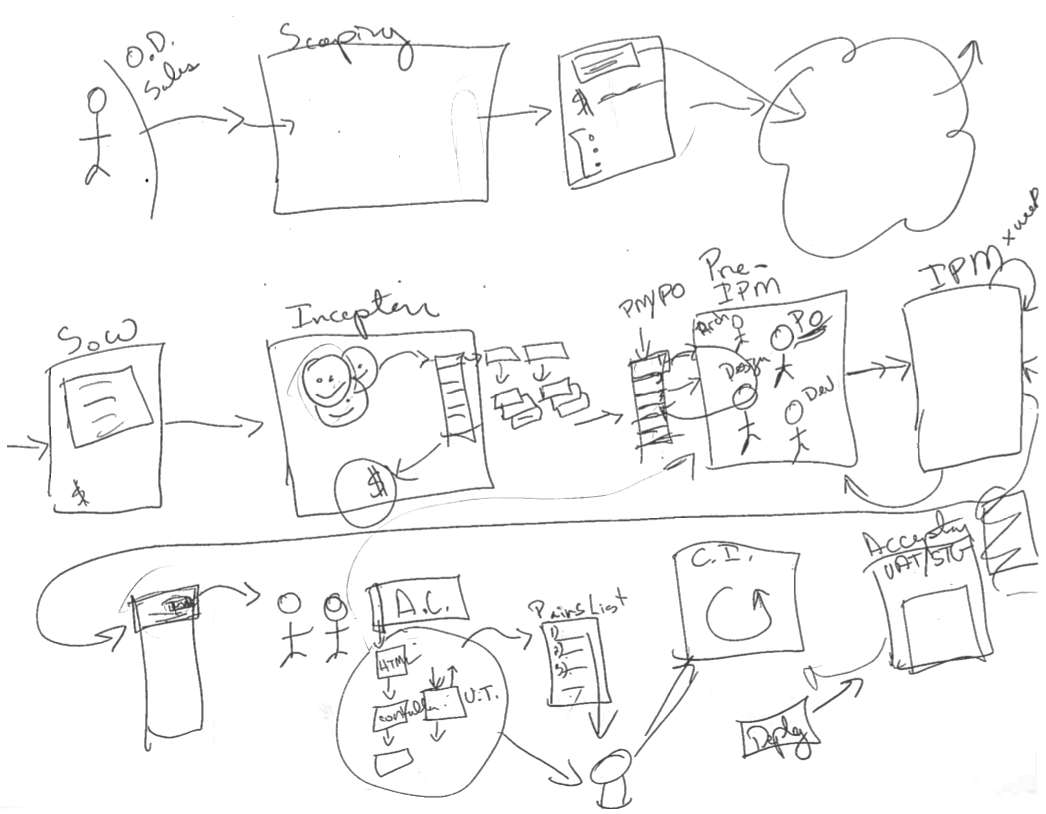
\includegraphics[width=\oneColumnWidth{}]{drawings/2015_08_12_anchor.png}
\caption{Interview 6: Detailed drawing of Pivotal's Software Development process}
\label{2015_08_12_detailed}
\end{figure}

When analysis shifted interviewing onto new topics, I would start with a new drawing question. For example, asking participants, \quotes{please draw your feelings about the code} often resulted in conversations about code ownership. Figure \ref{Interview31} shows an example. 

\begin{figure}[htbp]
\centering
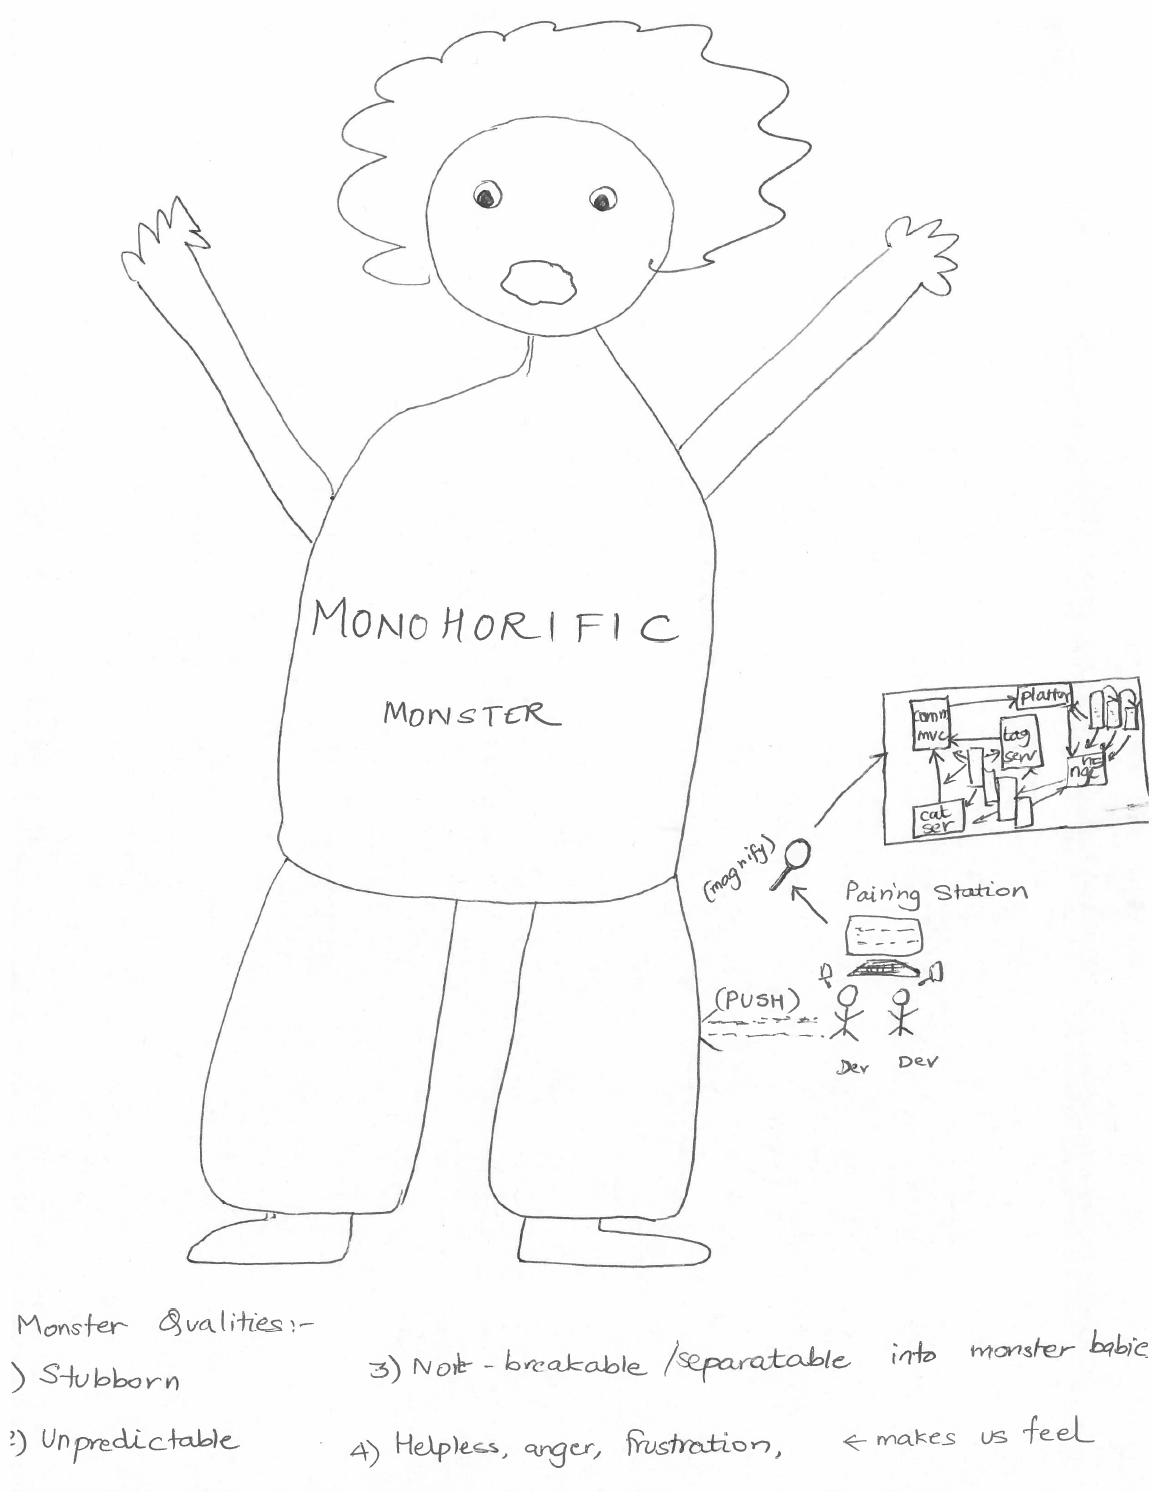
\includegraphics[width=\oneColumnWidth{}]{drawings/2016_09_26.png}
\caption{Interview 31: Software Engineer's drawing for \quotes{How you feel or how you think about the code'}}
\label{Interview31}
\end{figure}

\textit{Lesson Learned:} Asking participants to draw helped understand their perspective and provide a natural starting place for follow-up questions without forcing topics or perspectives.

\textit{Recommendation:} Try initiating interviews with a drawing question.

Meanwhile, I worked as a software engineer, on \numberOfObservedProjects{} sequential projects lasting \durationOfResearchStudyPlural{} (see \cite{SedanoSoftwareDevelopmentWaste} for details). I wrote extensive field notes on individual and collective actions, what participants found interesting or problematic, and emerging anecdotes and observations; for example: 

\participantQuote{Monday was the first time we started getting data from the client's servers. We've been implementing for several months without knowing whether our system would work with real backend systems. In order to make progress, we created mocks for each of the client's systems based upon documentation. Now we need to modify our code base to match the reality of the systems' implementation.}

\textit{Lesson Learned:} Collecting and analyzing field notes from participant observation is not easy. Just as Charmaz discovered that taking breaks from observation to write down her thoughts can be difficult \cite{Charmaz}, I found it very challenging to record observations during intensive activities (e.g. pair-programming). 

Participant observation provided a rich data for emergent ideas. For example, one day while pair programming, I realized that I did not know who was on my team because of significant team churn. This realization led me to convert task allocation data into a chart showing the start and stop dates for each team member, which raised the question, \textit{how was it possible to be successful \cite{RalphDimensionsOfSuccess} with the client with so many people rotating through the project?} Investigating this research question led to the Theory of Sustainable Software Development \cite{SedanoSustainableSoftware}.

\textit{Lesson Learned:} Participant observation often provided research insights not available from interviews or documents.

\textit{Recommendation:} Supplement interviews and document analysis with participant observation or direct observation (watching without interacting). Write detailed observations after work, but use post it notes or an unobtrusive notebook for capturing insights during intense activities. This was more culturally acceptable than typing on a laptop. Explain your actions to participants. For example, saying \quotes{I want to reflect on what you said} or \quotes{what you said was really insightful} makes the participant feel valued rather than ignored. In short breaks, try recording verbal notes; some phones will convert spoken words into text.
\section{Constant Comparison}
\label{ConstantComparison}
I used line-by-line coding \cite{Charmaz} to identify nuanced interactions in the data and avoid jumping to conclusions. Whenever insight occurred, I would write it down as a memo. My advisor reviewed the initial codes while reading the transcripts and listening to the audio recordings. We discussed the codes and the coding process during weekly research collaboration meetings. To avoid missing insights from these discussions \cite{GlaserTheoreticalSensitivity}, we often recorded and transcribed the discussion into Grounded Theory memos. As data was collected and coded, I stored initial codes in a spreadsheet and I used constant comparison to generate focused codes.

\textit{Lesson Learned:} I tend to continue too long with initial coding. 

\textit{Recommendation:} Use constant comparison to drive research forward.
\subsection{Understanding Constant Comparison}
Glaser's seminal book assumes the reader is a sociologist, making it inaccessible to many software engineering researchers and other non-sociologists. The term \textit{constant comparison} is especially challenging. Struggling to understand it---not just remember the definition but deeply understand how it works---I read three of Glaser's books \cite{GlaserDiscovery, GlaserIssues, GlaserTheoreticalSensitivity} and attended one of his seminars in Mill Valley, CA. The workshop helped me understand Grounded Theory terms that were not clear from the books. I later discovered clearer definitions \cite{GlaserBasics} (see Figure \ref{glaserDefinitions}), which Glaser wrote in response to Strauss and Corbin's \cite{Strauss1988Basics} criticisms.

\textit{Lesson Learned:} I needed to read four of Glaser's books and listen to him speak to properly understand constant comparison---Grounded Theory's main data analysis method. It involves continually comparing of codes to codes, codes to categories, codes within a category, and comparing categories to categories not only to generate and refine emerging theory but also to decide what data to collect next.

I routinely compared new codes to existing codes to refine codes and eventually generate categories. I periodically audited each category for cohesion by comparing its codes. When this comparison became complex, I printed codes on index cards, and then arranged and re-arranged until cohesive categories emerged. I wrote memos to capture the analysis of codes, examinations of theoretical plausibility, and insights.

\textit{Recommendation:} To deeply understand constant comparison, iterate between reading about grounded theory (or attending seminars) and analyzing your data. Accept that it takes study, practice and reflection to master. 


\begin{table}[t]
\renewcommand{\arraystretch}{1.5}
\centering
\captionof{figure}{Glaser's Definitions \cite{GlaserBasics} }
\label{glaserDefinitions}
\begin{tabular}{|l|}
\hline
\textit{Concept:} The underlying, meaning, uniformity and/or pattern within \\ a set of descriptive incidents. \\ 
\textit{Category:} A type of concept. Usually used for a higher level of \\ abstraction. \\
\textit{Property:} A type of concept that is a conceptual characteristic \\ of a category, thus at a lesser level of abstraction than a category. \\ A property is a concept of a concept. \\ 
\textit{Coding:} Conceptualizing data by constant comparison of incident \\ with incident, and incident with concept to emerge more categories and \\ their properties.
\\ \hline
\end{tabular}
\end{table}


\subsection{Pulling in new literature and data}
As the \textit{code ownership} category emerged, I looked to literature on ownership in general. Understanding the psychology of ownership \cite{Pierce2001} allowed me to connect team code ownership to underlying emotional needs and explained how emotions affect the transition from individual code ownership to team code ownership.

When \textit{removing waste} emerged as a topic, I examined Lean Software Development to understand how the Poppendiecks used the Toyota Production System waste taxonomy for software development \cite{PoppendieckConceptToCash}. Contrasting our emergent waste taxonomy with the Poppendiecks' top-down taxonomy helped us better understand and clarify its structure and elements. I also began collecting and analyzing data from retros. (A retrospection meeting (or retro) is a weekly meeting to collectively reflect on the work done during the week, i.e., a safe place where any team member can discuss any issue.) 

\textit{Lesson Learned:} Fortunately, I had been recording retro issues for over a year, so there was no waiting to gather the needed data. 

\textit{Recommendation:} Record easy to capture information, just in case. Take lots of photos.
\subsection{Dealing with Confusion}
During the analysis process, confusion can emerge. We found that sensemaking of comparing codes, naming concepts, defining terms, and identifying theoretical structure could be straightforward or anfractuous.

Glaser said that \quotes{confusion is the royal road to emergence,} \cite{GlaserMillValleyWorkshop}. 

My process for solving this tension looked like this:

\begin{enumerate}
  \item Be confused
  \item Try an idea (e.g. a name, a definition, a relationship between categories)
  \item Iterate on Step 2
  \item Experience an \quotes{Ah ha} moment
  \item Verify with data
\end{enumerate}

\textit{Lesson Learned:} Confusion appears to be a typical, critical step for the Grounded Theory researcher.

\textit{Recommendation:} Be patient, embrace the confusion.
\subsection{Focusing on a Manageable Topic}
For Glaser, a key matter is \quotes{what is the participant's main concern?} However, a study of this duration may produce several distinct core categories, necessitating ongoing scope adjustments. When my initial findings on course correcting seemed unwieldy, my co-advisor suggested that I focus on one concrete category at first. 

\textit{Lesson Learned:} Ambitious Grounded Theory studies can illuminate several interesting phenomena. For a novice, initially concentrating on one area helps drive constant comparison and theoretical sampling. Later, you can return to the other phenomena.

\textit{Recommendation:} When first learning Grounded Theory, focus on one emerging phenomenon of interest. 
\section{Theory Construction}
\label{TheoryConstruction}

The iterative process of constant comparison and memo-writing that generates a grounded theory may be straight-forward (as it was with our software development waste taxonomy), or confusing (as it was for the theory of sustainable software development). Understanding the relationship between properties may require significant analysis. For example, I grappled with the nature of the relationship between code ownership and teams thriving despite excessive churn. Does ownership encompass both ideas? No. Does surviving churn cover both ideas? Maybe. Are both concepts manifestations of the same more abstract phenomenon? No. After reviewing Glaser's 18 theoretical coding families, I reconceptualized surviving team churn as \quotes{sustainable software development} with team code ownership as one of its properties. 

We then started teasing apart the relationships between all the subcategories. Several felt different from each other. In time, we realized that some were practices, some were policies, and some were underlying principles. 

Refining the practices into clear, logical groups was difficult. We identified six practices that supported sustainable software development by supporting team code ownership. My advisor proposed a separation based on her reading the interview transcripts, but it did not resonate with the participant observation data. This spurred me into reconsidering the relationships between categories based on different specific questions. The question that eventually worked was, \quotes{which of these practices differently affect the code?} Three of them do. Then I asked \quotes{how are these other practices related?} They all concern knowledge silos. I recalled one interviewee discussing caretaking the code like a gardener and another expressing concern over knowledge silos forming on his team. I then labeled each group with \textit{in vivo} codes (phrases used by participants), leading to the \quotes{Caretaking the Code Practices} and \quotes{Removing Knowledge Silos Practices} categories. 

\textit{Lesson Learned:} The theoretical structure may take time to emerge.

\textit{Recommendation:} Review the 18 theoretical coding families in \underline{Theoretical Sensitivity} \cite{GlaserTheoreticalSensitivity}. However, do not adopt a coding family too readily---the coding family must earn its way into the theory like everything else.

Meanwhile, prior research treated code ownership as a team or organizational policy, whereas  our participants understood code ownership as an individual's feelings toward the code, further complicating matters. The progression in the memos is from \quotes{code ownership} to \quotes{communal code ownership}, \quotes{collective code possession} and eventually  \quotes{team code ownership} reflect my search for the best terms.

\textit{Lesson Learned:} Choosing the right names for emerging ideas is important and challenging.  

\textit{Recommendation:} When struggling with names, try \textit{in vivo} codes or terms used in existing literature. Try using variants in memos and conversations and see if any of them work. It is normal to feel conceptually uncomfortable during a Grounded Theory study. When in doubt, simply continue data collection and constant comparison.
\section{Theoretical Saturation}
\label{TheoreticalSaturation}
Once a theory emerged, the next question was \quotes{what more data do I need to collect?} Starting this research study, I thought I understood theoretical saturation. Eventually, I realized that I did not, and that the widely held definition of theoretical sampling as \quotes{the phase of qualitative data analysis in which the researcher has continued sampling and analyzing data until no new data appear and all concepts in the theory are well-developed} \cite{MorseTheoreticalSaturation} is problematic. 

Sampling until no new data emerges is subtly different than sampling to elaborate the emerging theory. 

Grounded Theory is not about repeating the same questions until they stop producing new information. The Grounded Theorist alters the questions based on the emerging data and asks new questions to help elaborate and corroborate the relationships between codes, between codes and categories, and between categories in the emerging theory. The process stops once the researcher is satisfied that the theory's concepts and relationships are mature and the theory feels whole. 

More data collection will often still reveal new concepts. The researcher may decide against including or further exploring these concepts for several reasons:
\begin{enumerate}
  \item The concept is not directly relevant to the current theory (out of scope).
  \item The concept has not earned its way into the theory. Potentially, a new Grounded Theory study at different site would be result in more incidents revealing that concept. 
  \item The concept represents a poor depth-to-parsimony tradeoff, that is, adding the concept would increase the theory's complexity without a reasonable corresponding increase in explanatory power. 
\end{enumerate}

In other words, the idea of no new data appearing is rooted in interview-focused, sociological research where interviewees just stop saying anything new. In participant-observation, software engineering research, we often have much more data than we can manually analyze, so \quotes{no new data} never happens. Researchers must use personal judgment and experience to recognize a saturated theory and halt data collection.   

At one point, I asked my advisor and co-advisor, \quotes{what questions should I ask my participants to achieve theoretical saturation?} This was unfair in retrospect. As the primary researcher, I am the one most qualified to know which relationships between the categories are not robust. I shifted from asking \quotes{what questions will get me theoretical saturation?} to asking myself, \quotes{what do I not know about this theory?}, \quotes{what is confusing?}, and \quotes{how do each of these categories relate?}

I finally understood Theoretical Saturation by reading and re-reading Charmaz and Glaser, experiencing saturation firsthand and discussing these challenges with my advisor and co-advisor. 

\textit{Lesson Learned:} Theoretical sampling is collecting additional data to develop full and robust categories, identify the relationships between categories, and elaborate the main category's properties.

\textit{Recommendation:} For saturation, focus on exploring and corroborating the emerging theory. Do not expect new data to dwindle.  
\section{Managing the Data}
\label{ManagingTheData}
During the study, I shifted from electronic to paper aids for constant comparison, as follows. 
\begin{enumerate}
  \item I initially did all constant comparison in Google spreadsheets
  \item I started hand-writing cards for hard-to-understand or complex comparisons and physically sorting them around me in a circle (e.g. needing to make sense of multiple perspectives about a backlog)
  \item I printed the codes directly related to team code ownership onto index cards
  \item I printed all the retrospective notes onto index cards
\end{enumerate}

When looking at rows in a spreadsheet, I found them blurring together and easy for me to gloss over. When holding a card, I felt compelled to consider it before putting it down. In a spreadsheet, I subconsciously felt that adjacent rows were related even when they were not. With physical cards, I found that picking up the next card helped me see it as something new. However, maintaining \textit{both} an electronic and physical copy was time consuming and felt wasteful.

The advantages of digital aids include:
\begin{itemize}
  \item Available wherever you have a computer
  \item Easy to share with co-authors
  \item Easy to backup and duplicate
  \item Simple to turn into physical cards
\end{itemize}

The advantages of physical aids include:
\begin{itemize}
  \item Easy to rearrange
  \item Easy to see big picture 
  \item Easy to focus on one area
  \item Easy to see outliers
  \item Easy to annotate with thoughts
  \item Encourages short capturing of ideas
  \item Time consuming to turn into electronic storage
\end{itemize}

\textit{Lesson Learned:} Sometimes using physical media can help with constant comparison. 

\textit{Recommendation:} There are many good ways to analyze data, and researchers need to find the techniques that work for them, but if you are getting lost in spreadsheets or NVivo, physical cards are worth trying.
\section{Publishing}
\label{Publishing}

I expected and experienced three main challenges with publishing this research. To the extent software engineering reviewers are familiar with Grounded Theory at all, they are accustomed to much shorter, interview-centric studies. Some of our reviewers did not understand analyses on data types (e.g. retrospective items) not usually used in Grounded Theory, or understand that such a long study produces multiple core categories, which cannot be addressed all in one paper. Meanwhile, some reviewers appear suspicious of qualitative research in general. To overcome their concerns, I distributed the methodology and findings very carefully across several interconnected papers. 

\textit{Lesson Learned:} It is extremely difficult to convey a large, participant-observation Grounded Theory study in a series of short papers, such that its methodological rigor is established and its findings are clear.

\textit{Recommendations:} Use existing guidance for presenting grounded theory to a software engineering audience \cite{StolGroundedTheory}. Rather than a long methods section, distribute ample methodological detail throughout the paper where appropriate. Explicitly address differences between interviews and participant observation. Clearly explain that you have conducted a \textit{long} study with several core categories, and that this paper only talks about this one category because space precludes treating all categories simultaneously. You can even cite our papers as precedent. Use a table or figure with examples to show the chain of evidence from raw data to categories. As reviewers, remember that the size of a competent grounded theory analysis precludes visualization even in a long journal article.
\section{Advantages and Disadvantages of Extended Participant Observation}
\label{AdvantagesDisadvantages}
Extended participant observation allows for a deep understanding of participants points of view. During this study, I have done almost 4,800 hours of pair programing. After thousands of conversations, I know what participants agree and disagree on. 

\textit{Lesson Learned:} Extended participant observation develops deep understanding of participant's perspective.

Many software engineering researchers began in the software development field because they enjoy writing software. Writing code with a development team exposes the researcher to the latest software development techniques employed in industry. A researcher who has experienced pair programming for several weeks may have a richer experience to draw upon than a researcher who has no pair programming experiences.

\textit{Lesson Learned:} Extended participant observation improves the researcher's technical skills, understanding of development processes, and empathy for software developers.

\textit{Recommendation:} Recognizing that it does not work for everyone, consider participant observation (or direct observation). Avoid over-reliance on interviews.

During extended, participant observation, promotion may present a dilemma. At one point, I was encouraged to apply for a promotion to Associate Director, a sales role with no time for coding. Because working directly with the teams was crucial for my research, getting this position would have derailed the study.. 

Furthermore, the research cycle gets complicated. When is the right time to present research findings? Would presenting research findings alter the system under study? I resolved these tensions by not withholding my opinions while pair programming, making decisions that were best for clients, my company, and my team. For example, I suggested adding retros to a team that was missing them, and for a struggling team, I introduced stress relieving measures and team building exercises.

The academic cycle of writing papers, submitting, resolving reviewer comments, and presenting the research is lengthy. Since Grounded Theory produces theories that are grounded in the observed context, we realized that sharing my published insights would not adversely affect my research. Giving my academic talks at Pivotal offices became a way for me to give back. 

\textit{Lesson Learned:} Sharing my published research with the organization resulted in lengthy helpful conversations. 

Moreover, business goals do not always align with the research goals. The research may be at the mercies of the business. Business needs dictated my rotation from team to team. Fortunately, most of my rotations enhanced my research, but I could be moved from a really interesting project to one with little research potential. At one point, I was even transferred to a different business unit. It did not undermine the research, but it could have. 

\textit{Lesson Learned:} Business decisions can have profound impacts on research. 

Glaser observed that Grounded Theory is easy to interrupt and pick up again. \quotes{Built into the method, is the ability to put it down at will and pick it up later with virtually no need to backtrack or unduly review where the researcher was before the break in pace. The study is always ready to go forward on the current, next step. Thus there is no need to sacrifice the requirements of and need for family, friends and recreation for the research. The research in progress is always there waiting to move forward when the researcher can return to it} \cite{GlaserIssues}. That said, balancing a 40-hour work week, research, and family is challenging. I kept saturdays free, and often used it for rest. 

\textit{Recommendation:} Build in rest time into your schedule.

As a developer, I have access to the stories in the backlog, daily conversations with my pair, team discussions, daily standups, weekly planning meetings, weekly retrospection meetings,  and the code itself. There is a lot of potential data to analyze---much more than just interviews. The retrospection dataset alone had 663 items. The volume of data can be overwhelming. I resonated with the saying, \quotes{a potential problem with ethnographic studies is seeing data everywhere and nowhere, gathering everything and nothing} \cite{Charmaz}. 

\textit{Recommendation:} Use the ideas emerging from constant comparison to guide what kinds of data to collect. 
\section{Conclusion}
\label{Conclusion}
This paper attempts to use my experience running an ambitious grounded theory study to illustrate some challenges and recommend some practices that I found helpful. Some of the key challenges are as follows:
Grounded Theory is more complicated than it first appears. I had to not only experience the method firsthand, but also read and re-read several seminal texts to really understand it.
Questions asking participant to draw a picture helped me focus on interviewees' perspectives and avoid forcing topics. 
Participant observation revealed many insights that interviews could not. 
Prioritizing analysis over data collection help me avoid getting overwhelmed.
My datasets were too unwieldy to analyze digitally; using physical index cards helped tremendously. 
Theoretical sampling is difficult to recognize and widely misunderstood. It is more about elaborating the emerging theory than running out of data. 
Extensive methodological detail and explicitly confronting the unusual aspects of the study helped assuage reviewer concerns. 

Glaser says that a Grounded Theory study can create a rich trove of data. Indeed, I am still collecting and analyzing data and there is much more here worth studying. If you are conducting a Grounded Theory study of your own, and especially if you are struggling, please feel free to contact me.

\section*{Acknowledgement}
Thank you to Rob Mee, David Goudreau, Ryan Richard, and Zach Larson for making this research possible.





